\documentclass{article}

\usepackage[utf8]{inputenc} % Use UTF-8 encoding
\usepackage{textgreek} % For Greek letters

\usepackage{algorithm}
\usepackage{algpseudocode}
\usepackage{hyperref}
\usepackage{fourier}
\usepackage{tikz}
\usepackage{array}

\DeclareMathAlphabet{\mathcal}{OMS}{cmsy}{m}{n}
\SetMathAlphabet{\mathcal}{bold}{OMS}{cmsy}{b}{n}
\newcommand{\bigO}{\mathcal{O}}

\begin{document}

\section{Introduction}
Sorting algorithms on modern computers have been playing an important role in Computer Science and can date back to the early 50s and 60s. 
It is the great efforts that humans have put into the field of developing faster sorting algorithms that shapes the vital parts that formed
all the significant infrastructures of the vast computer world like databases, data centers, cluster networks etc.
In the realm of sorting algorithms, Quicksort, introduced by computer scientist Tony Hoare \cite{HoareQuickSort} to the public,
has made its way into the libc of the GNU/Linux system and stood the test of time as one of the most classical and widely used methods for sorting. 
Its divide-and-conquer strategy has been widely used and taken into research to fully utilize the performance of sorting.
The basic Quicksort picks an arbitrary pivot element,
partitions the array into 2 segments, one with elements less than the pivot and the other greater. 
It then recursively sorts these segments using the same method. While the original Quicksort method has proven effective,
the quest of further optimizations and the endless pursuit of efficiency has led to many variations to explore, one of which is the Multi-Pivot Quicksort. 

This thesis is my shallow attempt to unveil the benefits of Multi-Pivot Quicksort, exploring the effects more pivots can bring,
followed by some potential implementations and the analysis on the benefits that arise from leveraging multiple pivots in the Quicksort process.

\subsection{History and Related work} 

When Quicksort was first invented a great number of variations and modifications were put into research over the years, 
such as sorting with a better partition method and a more optimal strategy to select the arbitrary pivot element.
But the innovative approach of Multi-pivot Quicksort, exemplified by Vladimir Yaroslavskiy \cite{Yaroslavskiy} in 2009,
Bentley and Bloch's algorithm, which was also highlighted by Wild and Nebel, adopted in Sun's Java 7 runtime library, 
introduces the use of two pivots. Contrary to initial expectations, studies have revealed that employing multiple pivots can enhance the performance,
challenging prior assumptions derived from the dual-pivot proposal by Sedgewick \cite{Sedgewick} in 1978 where he analyzed a potential dual-pivot approach, 
which was deemed inferior to the classical Quicksort in his research. Furthermore, Kushagra presented a 3-pivot Quicksort \cite{Kushagra} algorithm at ALENEX,
has attracted significant attention, further pushing the researches of multi-pivot strategies. 

One common pitfall in the performance downgrade of the conventional Quicksort is the degenerated cases,
which could often arise when the input array is already mostly sorted or when certain patterns in the data cause the algorithm to consistently choose poor pivots
that fail to split the data into evenly sized partitions. 
In such cases, the partitioning process may result in highly unbalanced partitions, leading to suboptimal performance and
potentially degrading the time complexity to $\bigO(n^2)$ instead of the expected $\bigO(n\log n)$ for Quicksort.
Wiser choices of pivot selections could decrease the possiblities of such events from happening, such as the median-of-3 method and its variations of median-of-5 and median-of-7.
But on mostly ascending or descending arrays, the median-of-3 method still has a chance of choosing the smallest or largest element as the pivot,
which is not the best ideal approach to prevent the worst case from happening. It also brings to our concerns that in real world applications, duplicated elements are not rare,
and the median-of-3 method could be easily affected by the duplicated elements, which could lead to the same worst case as the original Quicksort. 
There are some other variations of Quicksort that have been proposed to address these specific issues, such as the Introsort algorithm \cite{Introsort} by David Musser,
which switches to Heapsort when the recursion depth exceeds a certain threshold. Thus the worst running time is guaranteed to be $\bigO(n\log n)$ by doing so.

And this is where Multi-pivot quicksort comes into play. Assuming we are dealing with randomly generated arrays,
since we don't know the exact size of each partition, the more pivots we choose, the more partitions we divide the array into,
the less chance it will be that we encounter imbalanced sizes of partitions. 
Moreover, choosing more pivots will significantly reduce the chance we access the same elements again and the maximum depth of recursion,
which can translate into better running time. With n pivots we are dividing the array into n+1 partitions, the same things happen on the sub-partitions 
in the next level of recursion and we can conclude the maximum depth of recursion would be $\log_{n+1} L$ given \textbf{n} as the number of pivots and \textbf{L} for the length of array.
Greater the n is, less the depth. Better memory behaviors can bring effects that can not be achieved by any of other traditional means such as choosing a better pivot value
among samples extracted from different parts of the array, but the drawbacks are also obvious, 
branch misprediction could be terrible as the different outcomes of comparisons can largely impact on the runtime performance.
A delay of 14 to 19 stages on a typical Intel desktop CPU or 20 to 25 stages on AMD's Zen CPUs could lead to huge efficiency loss for our algorithm,
and this number only grows as the number of pivots increases and on more complicatad architectures. These are the trade-offs we have to consider when we are choosing the number of pivots,
although these side effects can be mitigated by the use of branchless comparisons and modern CPUs are able to run conditional move operations (cmove) to avoid branches,
these overheads still remain as concerns.
Apart from that, it could be really tricky when it comes to moving the elements to the right places among multiple partitions, especially when the number of pivots is large.
Additionally, comparisons are the second expensive things next to swaps we are dealing with, and the more pivots we choose, the more comparisons we have to make.
Even for the case of using only one pivot, the average number of comparisons remain unoptimial, being $1.38n\log n + \bigO(n)$ compared with the $n\log n + \bigO(n)$ of the Merge Sort,
but the overall instructions are much less than the average of Merge Sort and with proper pivot selection strategy, it can still be reduced to a certain extent.

% As the number of pivots increase, it is important that we take the worst cases into consideration. 
% Will we end up wasting too much time on comparing with badly-chosen similar pivots that split the array into imbalanced partitions,
% one of which might have much larger size than the rest? Or Even with the relatively higher amount of branch mispredictions, 
% will we still conquer the barriers of cache misses caused by long-lasting swaps of elements far away and reach a shorter time as the n grows?
% That's the riddle I'm going to research in the next section.

Fortunately, an efficient approach has been put forward by Stefan Edelkamp and Armin Weiß,
in their thesis of BlockQuickSort \cite{BlockQuickSort}
which evens the odds of both branch mis-prediction and cache misses which uses one or more buffer blocks of constant sizes on the stack
to store the index offsets of out-of-order elements, swap them altogether in a second pass to rearrange them in order
after scanning a large chunk of array with the size of the block. Their approach realized a significant speedup up to 80\% faster compared with the GCC implementation of std sort
with only one single pivot. The BlockQuickSort has been adapted to the Multi-Pivot Quicksort and the results are also promising,
the improvements on contiguous memory access significantly improves the spatial locality and reduces both the cache misses and branch mis-predictions.
Branchless comparisons are also adapted which plays an important role in contributing to the huge performance boost by reducing the overhead
when increasing the counter of elements stored in the block buffer(s).
This novel approach has also developed variations that could effectively make the use of different partitioning methods and multiple pivots selected. 

Meanwhile, in the pursuit of advancing the efficiency of the Quicksort algorithm,
my investigation led me to explore various modifications, 
with a particular focus on the pattern-defeating Quicksort (PDQSort) proposed by Orson Peters. 
PDQSort leverages the average-case performance of randomized Quicksort with the rapid worst-case execution of heapsort, 
while concurrently achieving linear time complexity for slices exhibiting specific patterns. 
Notably, PDQSort employs a judicious application of randomization to prevent the degenerated case from happening.
When it does, PDQSort will strategically shuffle or reverse the entire array to simplify the sorting and increase the speed.
If all the counter measures fail, it also has the final backup plan of switching to Heapsort when bad choices of pivots or the depth of recursions exceed the limit. 
In terms of pivot selection, it uses a fixed seed when generating a pseudo-random index to ensure the reproducibility and deterministic behavior.
Furthermore, in instances where randomly selected elements from the original array appear in a descending order.
The combination of these optimizations has demonstrated a significant enhancement in performance, showcasing PDQSort as up to twice faster than the original Quicksort algorithm. 
This outcome illuminates the transformative impact that a comprehensive analysis on the pattern of arrays has on the speed of sorting algorithms,
not to mention it is a successful combination of BlockQuickSort's partition method,
Heap sort when dealing with worst cases and Insertion sort when it comes to small sub-arrays of sizes less than the cache line size. 
Inspired by PDQSort's success, I dive into the diverse variations of Quicksort,
motivating a search for novel patterns that may be leveraged to enhance the existing Quicksort algorithms.

\subsection{Contributions}
\begin{itemize}
    \item Present the variants of Multi-Pivot QuickSort and implement a 4-Pivots Quicksort and evaluate N-Pivots Quicksort from N = 1, 2, 3, 4 experimentally. 
        Comparing the implementations, times, instructions, cache misses and branch mis-predictions with a duration of 3 seconds warm-up time.
    \item Present a new layout of Multi-Pivot BlockQuickSort that could potentially reduce the memory access and increase the block buffer usage rate. 
        Analyze this method with all other available variants with block partitioning and compare the pros and cons.
\end{itemize}

\section{Preliminaries}
\begin{algorithm}[H]
    \caption{QuickSort with Hoare Partition}\label{HoarePartition}
    \begin{algorithmic}[1]
        \Procedure{QuickSort}{$A, l, r$}
        \If{$l < r$}
        \State $p \gets \textsc{HoarePartition}(A, l, r)$
        \State \textsc{QuickSort}(A, l, p-1)
        \State \textsc{QuickSort}(A, p+1, r)
        \EndIf
        \EndProcedure
        \Procedure{HoarePartition}{$A, l, r$}
        \State $P \gets A[l]$ \Comment{Pivot}
        \State $i \gets l - 1$
        \State $j \gets r + 1$
        \While{$i < j$}
        \Repeat
        \State $j \gets j - 1$
        \Until{$A[j] < P$}
        \Repeat
        \State $i \gets i + 1$
        \Until{$A[i] > P$}
        \State \textsc{Swap}($A[i], A[j]$)
        \EndWhile
        \State \textsc{Swap}($A[l], A[j]$) \Comment{Put pivot in the middle}
        \State \textbf{return} $j$
        \EndProcedure
    \end{algorithmic}
\end{algorithm}

For Quicksorts with single pivot value, the partitioning procedure splits the array into 2 parts where the left part are elements less than the pivot and the right part being greater, 
separated by the pivot value in the middle. Then the main body recursively sorts the left and right part to rearrange all the elements in the correct order. The hoare's partition method
uses double pointers starting at the leftmost and the rightmost element in the array and scanning towards the middle until they meet. Each pointer scans for mis-placed elements 
which belong to the other partition by comparing the current element to the pivot. 
Out-of-order elements are swapped in pairs to the right place and the scanning procedure continues until all elements 
are moved to the places where they belong.

\begin{algorithm}[H]
    \caption{QuickSort with Lomuto Partition}\label{LomutoPartition}
    \begin{algorithmic}[1]
        \Procedure{QuickSort}{$A, l, r$}
        \If{$l < r$}
        \State $p \gets \textsc{LomutoPartition}(A, l, r)$
        \State \textsc{QuickSort}(A, l, p-1)
        \State \textsc{QuickSort}(A, p+1, r)
        \EndIf
        \EndProcedure
        \Procedure{LomutoPartition}{$A, l, r$}
        \State $P \gets A[r]$ \Comment{Pivot}
        \State $i \gets l$
        \For{$j \gets l$ \textbf{to} $r-1$}
        \If{$A[j] < P$}
        \State \textsc{Swap}($A[i], A[j]$)
        \State $i \gets i + 1$
        \EndIf
        \EndFor
        \State \textsc{Swap}($A[i], A[r]$) \Comment{Put pivot in the middle}
        \State \textbf{return} $i$
        \EndProcedure
    \end{algorithmic}
\end{algorithm}

While the Lomuto partition method uses another way, it scans the array in sequential order from left to right using one bare pointer
and swaps all the elements less than the pivot to the left side regardless,
thus duplicated swaps are introduced due to not checking if the elements are already in the right places. Both of these 2 partition methods are straightforward, 
and their main structures are similar: scan, find mis-placed elements, swap and recursively repeat the same procedure until the whole array is sorted.

\begin{algorithm}[H]
    \caption{Dual-Pivot QuickSort}\label{DualPivotQuickSort}
    \begin{algorithmic}[1]
        % \Procedure{DualPivotQuickSort}{$A, l, r$}
        % \If{$l < r$}
        % \State $p1, p2 \gets \textsc{DualPivotPartition}(A, l, r)$
        % \State \textsc{DualPivotQuickSort}(A, l, p1-1)
        % \State \textsc{DualPivotQuickSort}(A, p1+1, p2-1)
        % \State \textsc{DualPivotQuickSort}(A, p2+1, r)
        % \EndIf
        % \EndProcedure

        \Procedure{DualPivotPartition}{$A, l, r$}
        \State $P1, P2 \gets A[l], A[r]$ \Comment{Pivots}
        \If{$P1 > P2$}
        \State \textsc{Swap}($P1, P2$)
        \EndIf

        \State $less \gets l + 1$
        \State $greater \gets r - 1$

        \State $k \gets l$
        \While{$k \leq greater$}
            \If{$A[k] < P1$} \Comment{If the current element is less than P1}
                \State \textsc{Swap}($A[k], A[less]$) \Comment{Shift the element to the leftmost partition}
                \State $less \gets less + 1$
            \ElsIf{$A[k] > P2$} \Comment{If the current element is greater than P2}
                \While{$A[greater] > P2$ \textbf{and} $k < greater$}
                    \State $greater \gets greater - 1$ \Comment{Find the first element less than P2}
                \EndWhile
                \State \textsc{swap}(A[k], A[greater]) \Comment{Swap to the rightmost partition}
                \State $greater \gets greater - 1$
    
                \If{$A[j] < P1$} \Comment{Double check if another swap is needed}
                    \State \textsc{Swap}($A[k], A[less]$) 
                    \State $less \gets less + 1$
                \EndIf
            \EndIf
            \State $k \gets k + 1$ \Comment{Move to the next element}
        \EndWhile
        \State $less \gets less - 1$
        \State $greater \gets greater + 1$
        \State \textsc{Swap}($A[l], A[less]$) \Comment{Put Pivot1 in the middle}
        \State \textsc{Swap}($A[r], A[greater]$) \Comment{Put Pivot2 in the middle}
        \State \textbf{return} $less, greater$
        \EndProcedure
    \end{algorithmic}
\end{algorithm}

With one more pivot added, the two-pivot Quicksort method is introduced by Vladimir Yaroslavskiy in 2009. It uses 2 pivots selected from each end to split the array into 3 parts.
K stands for the current element being scanned, it will be swapped to the left part, which is accumulated by the less pointer, if it is less than the first pivot or do nothing if it is in the middle part.
Otherwise, if it is greater than the second pivot, it will be swapped to the right part, which is accumulated by the greater pointer.
We will double check the current element at index k after the swap to see if it is less than the first pivot, if so, we will swap it to the left part and move the less pointer to the right.
Hereby, we can see that the Dual-Pivot Quicksort is a generalization of the original Quicksort, and the partitioning method is also a generalization of the original Hoare's partition method but with 2 pivots.

\begin{algorithm}[H]
    \caption{3-Pivot QuickSort}\label{3PivotQuickSort}
    \begin{algorithmic}[1]
        \Procedure{ThreePivotPartition}{$A, l, r$}
        \State $P1, P2, P3 \gets A[l], A[l+1], A[r]$ \Comment{And sort 3 Pivots in ascending order} 

        \State $i, j \gets l + 2$
        \State $k, l \gets r - 1$
        \While{$j \leq k$}
            % // j moves right until arr[j] >= p2
            % while arr[j].cmp(&p2) == Ordering::Less {
            %     // arr[<i] -> elements that are less than p1, arr[i] is not less than p1
            %     if arr[j].cmp(&p1) == Ordering::Less {
            %         arr.swap_unchecked(i, j);
            %         i += 1;
            %     }
            %     j += 1;
            % }
            \While{$A[j] < P2$} \Comment{Put left side elements less than P2 in order}
                \If{$A[j] < P1$}
                    \State \textsc{Swap}($A[i], A[j]$)
                    \State $i \gets i + 1$
                \EndIf
                \State $j \gets j + 1$
            \EndWhile
            % // k moves left until arr[k] <= p2
            % while arr[k].cmp(&p2) == Ordering::Greater {
			% 	// arr[>l] -> elements that are greater than p3, arr[l] is not greater than p3
			% 	if arr[k].cmp(&p3) == Ordering::Greater {
			% 		arr.swap_unchecked(k, l);
			% 		l -= 1;
			% 	}
			% 	k -= 1;
			% }
            \While{$A[k] > P2$} \Comment{Put right side elements greater than P2 in order}
                \If{$A[k] > P3$}
                    \State \textsc{Swap}($A[k], A[l]$)
                    \State $l \gets l - 1$
                \EndIf
                \State $k \gets k - 1$
            \EndWhile
			% // if j is still less than k
			% if j <= k {
			% 	if arr[j].cmp(&p3) == Ordering::Greater {
			% 		if arr[k].cmp(&p1) == Ordering::Less {
			% 			// if arr[j] > p3 and arr[k] < p1, 
			% 			// rotate arr[j] to k and arr[k] to i because arr[<i] < p1
			% 			rotate3(arr, [j, i, k]);
			% 			i += 1;
			% 		} else {
			% 			// if arr[j] > p3 and arr[k] >= p1,
			% 			// simply swap arr[j] and arr[k]
			% 			arr.swap_unchecked(j, k);
			% 		}
			% 		// at this moment arr[k] must be greater than p3
			% 		// swap it with arr[l] to move it to the right
			% 		arr.swap_unchecked(k, l);
			% 		l -= 1;
			% 	} else { 
			% 		// if arr[j] <= p3, we do the same logic as above
			% 		if arr[k].cmp(&p1) == Ordering::Less {
			% 			rotate3(arr, [j, i, k]);
			% 			i += 1;
			% 		} else {
			% 			arr.swap_unchecked(j, k);
			% 		}
			% 		// at this moment arr[j] must be less than or equal p1
			% 		// arr[k] must be less than or equal p3
			% 	}
			% 	j += 1;
			% 	k -= 1;
			% }
            \If{$j \leq k$}
                \If{$A[j] > P3$} \Comment{Deal with 2 branches when A[j] is greater than P3}
                    \If{$A[k] < P1$}
                        \State \textsc{Rotate3}($A, [j, i, k]$)
                        \State $i \gets i + 1$
                    \Else
                        \State \textsc{Swap}($A[j], A[k]$) \Comment{A[j] > P3 and P2 > A[k] $\ge$ P1}
                    \EndIf
                    \State \textsc{Swap}($A[k], A[l]$)
                    \State $l \gets l - 1$
                \Else \Comment{Deal with 2 branches when A[j] is less than or equal to P3}
                    \If{$A[k] < P1$}
                        \State \textsc{Rotate3}($A, [j, i, k]$)
                        \State $i \gets i + 1$
                    \Else
                        \State \textsc{Swap}($A[j], A[k]$)
                    \EndIf
                \EndIf
                \State $j \gets j + 1, k \gets k - 1$
            \EndIf
        \EndWhile
        \State $i \gets i - 1, j \gets j - 1, k \gets k + 1, l \gets l + 1$
        % rotate3(arr, [left + 1, i, j]);
        \State \textsc{Rotate3}($A, [left + 1, i, j]$)
        % arr.swap_unchecked(left, i);
		% arr.swap_unchecked(right, l);
        \State \textsc{Swap}($A[left], A[i]$)
        \State \textsc{Swap}($A[right], A[l]$)
        \State \textbf{return} $i, j, l$
        \EndProcedure
    \end{algorithmic}
\end{algorithm}


The three-pivot Quicksort, introduced by Shrinu Kushagra, uses the similar hoare-like partition method, is a further generalization of the Dual-Pivot Quicksort.
In the original implementation, the 3 pivots are selected from the leftmost, the second element and the rightmost element of the array, and are sorted in ascending order.
The scanning procedure is similar to the Dual-Pivot Quicksort, but with 3 pivots, the array is divided into 4 parts, and is repeated until all elements are set.
The i, j, k, l pointers are used to scan the array and the elements are swapped to the right places according to the comparison results with the 3 pivots,
where i stands for the leftmost part where elements less than Pivot 1 belongs, j stands for the middle-left part, k stands for the middle-right part and l stands for the rightmost part.
Between j and k stands the unknown region where elements are not yet compared with any of the pivots. 
If the elementa at index j is less than Pivot 2, it is whether swapped to the leftmost part if it is less than Pivot 1,
or do nothing otherwise, since the middle-left part is for elements greater than Pivot1 and less than or equal to Pivot 2.
Same logic applies to the rightmost part, where elements are greater than Pivot 2 and less than or equal to Pivot 3.
These two pre-conditions are checked before the main body of the swapping and rotating procedure, which corresponds to the 2 while loops applied at the top of the main scanning loop.
Afterwards, the real swapping and rotating procedure is applied to the elements at index j and k, which are on the left and right boundaries of the unknown region, need to go to the other side of the array and moved to the right places.
We can simplify this part into a 2 if-else nested block, where the outter if-else block is for the case at index j and the inner one is for the case at index k.
Both of them have 2 branches, one for the case where the current element belongs to the leftmost or the rightmost part, and the other for the case where it belongs to the middle-left or the middle-right part.
It is not hard to tell there are $2 \times 2 = 4$ branches in total, and the swapping and rotating procedure is applied to each of them. The following chart \hyperlink{fig:3pivot}{*} illustrates the 4 branches and the corresponding actions.

% \listoffigures
\begin{figure}[H]
    \hypertarget{fig:3pivot}{}
    \caption{3-Pivot Quick Sort}
    \centering
    \hspace*{-0.25\textwidth}
    % \vspace*{+0.1\textheight}
    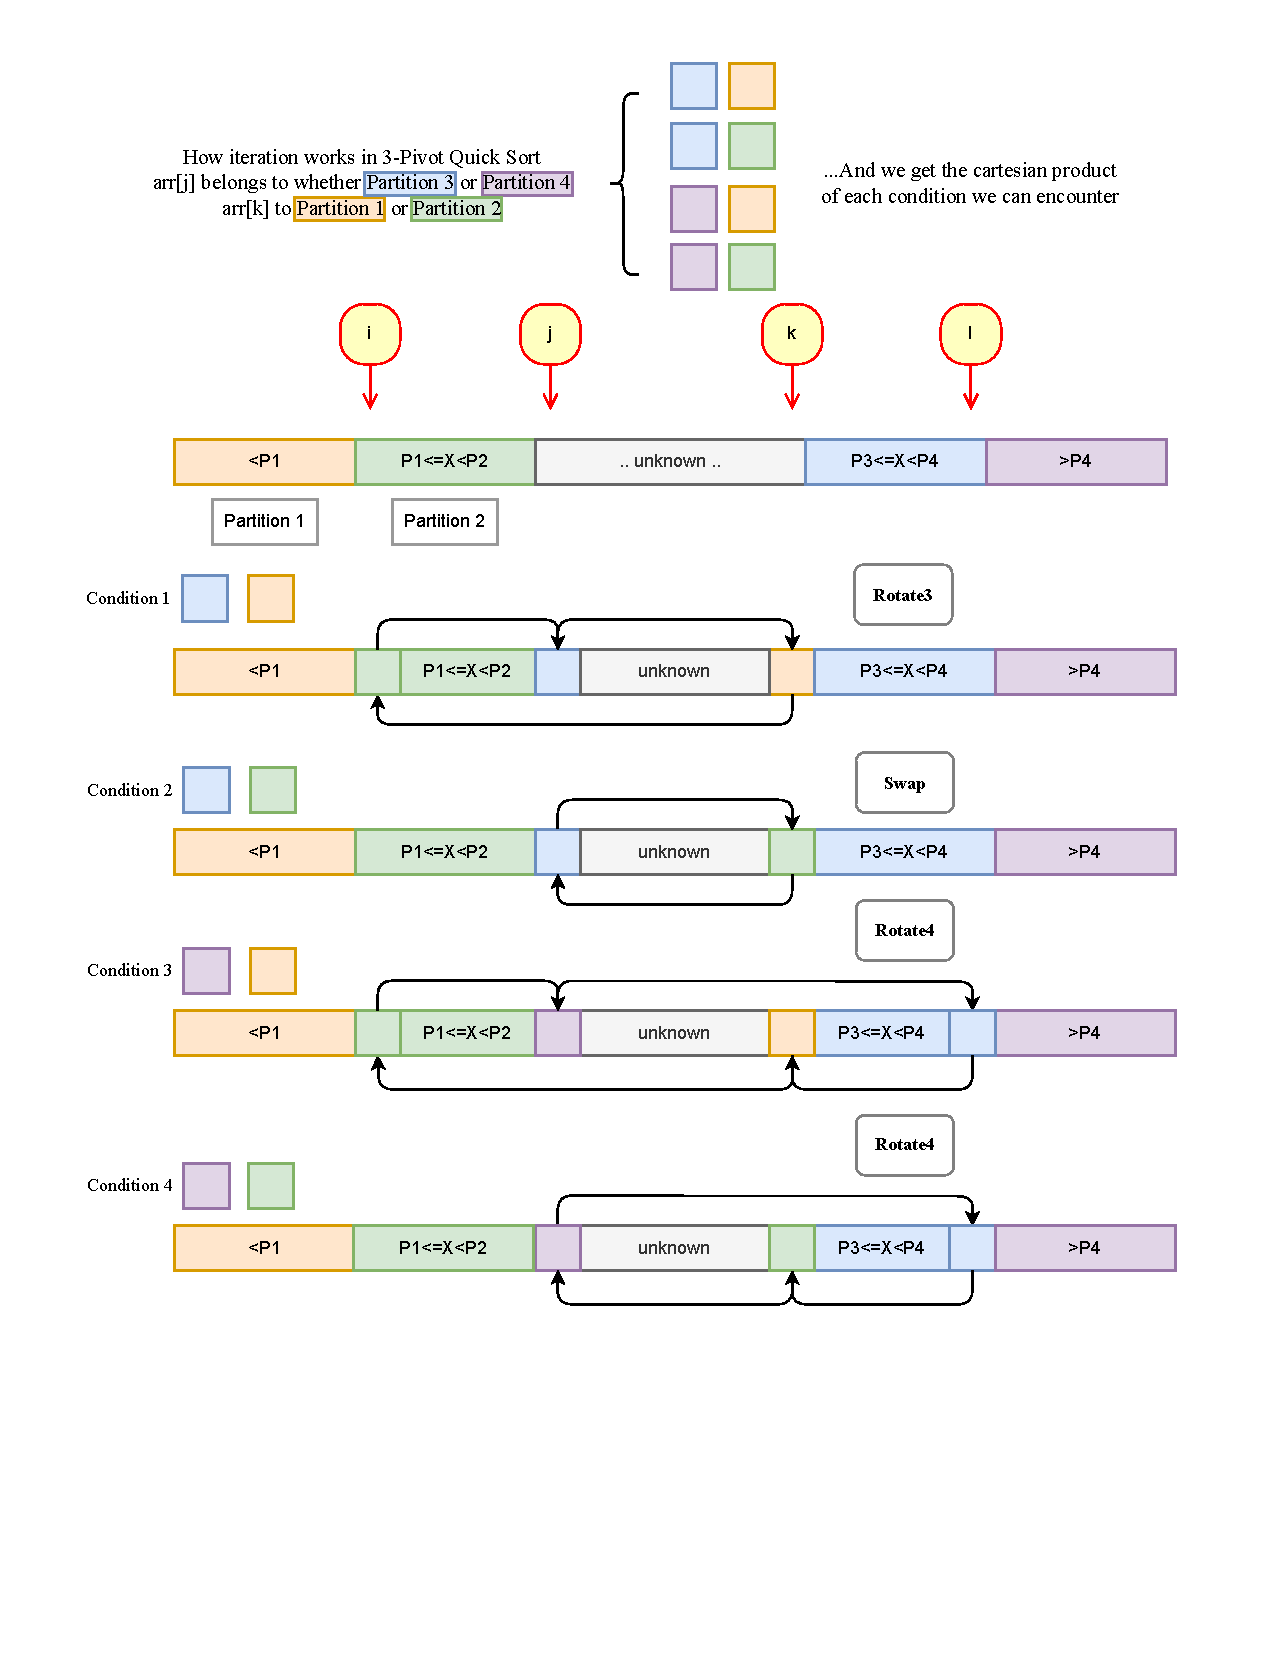
\includegraphics[width=1.5\textwidth]{3pivot.drawio.pdf}
\end{figure}

\begin{algorithm}[H]
    \caption{4-Pivot QuickSort}\label{4PivotQuickSort}
    \begin{algorithmic}[1]
        \Procedure{FourPivotPartition}{$A, l, r$}
        
        % let p1: *mut T = &mut arr[left];
		% let p2: *mut T = &mut arr[left + 1];
		% let p3: *mut T = &mut arr[right - 1];
        % let p4: *mut T = &mut arr[right];
        \State $P1, P2, P3, P4 \gets A[l], A[l+1], A[r-1], A[r]$ \Comment{And sort 4 Pivots in order} 

        % let (mut i, mut j, mut k, mut l, mut m) = (left + 2, left + 2, left + 2, right - 2, right - 2);
		% let (p1, p2, p3, p4) = (ptr::read(p1), ptr::read(p2), ptr::read(p3), ptr::read(p4));
        

        % while k <= l {
        %     //        | i              | j              | k
        %     // | < p1 | >= p1 and < p2 | >= p2 and < p3 | unknown
        %     while arr[k].cmp(&p3) == Ordering::Less {
        %         if arr[k].cmp(&p1) == Ordering::Less {
        %             rotate3(arr, [k, j, i]);
        %             i += 1;
        %             j += 1;
        %         } else if arr[k].cmp(&p2) == Ordering::Less {
        %             arr.swap_unchecked(k, j);
        %             j += 1;
        %         }
        %         k += 1;
        %     }
        \State $i, j, k, l, m \gets l + 2, l + 2, l + 2, r - 2, r - 2$
        \While{$k \leq l$}
            \While{$A[k] < P3$} \Comment{Put left side elements less than P3 in order}
                \If{$A[k] < P1$}
                    \State \textsc{Rotate3}($A, [k, j, i]$)
                    \State $i \gets i + 1$, $j \gets j + 1$
                \ElsIf{$A[k] < P2$}
                    \State \textsc{Swap}($A[k], A[j]$)
                    \State $j \gets j + 1$
                \EndIf
                \State $k \gets k + 1$
            \EndWhile
            % //        | l              | m              | 
            % // | >= p3 and < p4 | unknown
            % while arr[l].cmp(&p3) == Ordering::Greater {
            %     if arr[l].cmp(&p4) == Ordering::Greater {
            %         arr.swap_unchecked(l, m);
            %         m -= 1;
            %     }
            %     l -= 1;
            % }
            \While{$A[l] > P3$} \Comment{Put right side elements greater than P3 in order}
                \If{$A[l] > P4$}
                    \State \textsc{Swap}($A[l], A[m]$)
                    \State $m \gets m - 1$
                \EndIf
                \State $l \gets l - 1$
            \EndWhile
        %     if k <= l {
        %         if arr[k].cmp(&p4) == Ordering::Less {
        %             // arr[k] > p3, arr[l] < p3
        %             if arr[l].cmp(&p1) == Ordering::Less {
        %                 rotate4(arr, [k, j, i, l]);
        %                 i += 1;
        %                 j += 1;
        %             } else if arr[l].cmp(&p2) == Ordering::Less {
        %                 rotate3(arr, [k, j, l]);
        %                 j += 1;
        %             } else {
        %                 arr.swap_unchecked(k, l);
        %             }
        \If {$k \leq l$} \Comment{Start manipulation on the boundaries of unknown region}
            \If{$A[k] < P4$} \Comment{Deal with 3 branches when A[k] is less than P4}
                \If{$A[l] < P1$}
                    \State \textsc{Rotate4}($A, [k, j, i, l]$)
                    \State $i \gets i + 1$, $j \gets j + 1$
                \ElsIf{$A[l] < P2$}
                    \State \textsc{Rotate3}($A, [k, j, l]$)
                    \State $j \gets j + 1$
                \Else
                    \State \textsc{Swap}($A[k], A[l]$)
                \EndIf
        %         } else {
        %             // arr[k] > p4, arr[l] < p3
        %             if arr[l].cmp(&p2) == Ordering::Greater { // arr[l] goes to (p2, p3), increase k
        %                 rotate3(arr, [k, l, m]);
        %             } else if arr[l].cmp(&p1) == Ordering::Greater { // arr[l] goes to (p1, p2), increase j and k
        %                 rotate4(arr, [k, j, l, m]);
        %                 j += 1;
        %             } else { // arr[l] goes to leftmost side
        %                 rotate5(arr, [k, j, i, l, m]);
        %                 i += 1;
        %                 j += 1;
        %             }
        %             m -= 1;
        %         }
        %         k += 1;
        %         l -= 1;
        %     }
        % }
            \Else \Comment{Deal with 3 branches when A[k] is greater than P4}
                \If{$A[l] > P2$}
                    \State \textsc{Rotate3}($A, [k, l, m]$)
                \ElsIf{$A[l] > P1$}
                    \State \textsc{Rotate4}($A, [k, j, l, m]$)
                    \State $j \gets j + 1$
                \Else
                    \State \textsc{Rotate5}($A, [k, j, i, l, m]$)
                    \State $i \gets i + 1$, $j \gets j + 1$
                \EndIf
                \State $m \gets m - 1$
            \EndIf
            \State $k \gets k + 1$, $l \gets l - 1$
        \EndIf
        \algstore{4pivots}
    \end{algorithmic}
\end{algorithm}

\clearpage

\begin{algorithm}[H]
    \caption{4-Pivot QuickSort (Continued)}\label{4PivotQuickSort2}
    \begin{algorithmic}[1]
        \algrestore{4pivots}
        \EndWhile
        % i -= 1;
        % j -= 1;
        % // k -= 1;
        % l += 1;
        % m += 1;
        \State $i \gets i - 1, j \gets j - 1, k \gets k - 1, l \gets l + 1, m \gets m + 1$
        % // i, j, l, m are indexes of pivot 1, 2, 3, 4
        % // Here is the place rotate3 can't be replaced by arr.rotate_left
        % // because the indexes (left + 1 > i ?) are not always ascending
        % // so it could lead to a panic
        % // anyway, I leave the rotate_n macro for you to try out in `src/util.rs`
        % rotate3(arr, [left + 1, i, j]);
        % i -= 1;
        % arr.swap_unchecked(left, i);
        
        % rotate3(arr, [right - 1, m, l]);
        % m += 1;
        % arr.swap_unchecked(right, m);
        \State \textsc{Rotate3}($A, [left + 1, i, j]$)
        \State $i \gets i - 1$
        \State \textsc{Swap}($A[left], A[i]$)
        \State \textsc{Rotate3}($A, [right - 1, m, l]$)
        \State $m \gets m + 1$
        \State \textsc{Swap}($A[right], A[m]$)
        \EndProcedure
    \end{algorithmic}
\end{algorithm}

As long as the number of pivots increases, the number of branches will grow linearly, and the complexity of the partitioning method will also increase.
Thankfully, for 4-Pivot QuickSort \hyperlink{fig:4pivot}{*}, we are just adding two more branches (As showed in the blue-red and purple-red branches in the chart below)
into considerations and the branching logic is still under control.
It is for sure that we are going to have 9 branches for 5-Pivot QuickSort (3 partitions on each side, $3 \times 3 = 9$) and 12 branches for 6-Pivot QuickSort (3 partitions on one side and 4 on the other, $3 \times 4 = 12$).
The complexity of the partitioning method is growing way too far and thus only 4-Pivot QuickSort will be discussed in this thesis.

\begin{figure}[H]
    \hypertarget{fig:4pivot}{}
    \caption{4-Pivot Quick Sort}
    \centering
    \hspace*{-0.25\textwidth}
    % \vspace*{+0.1\textheight}
    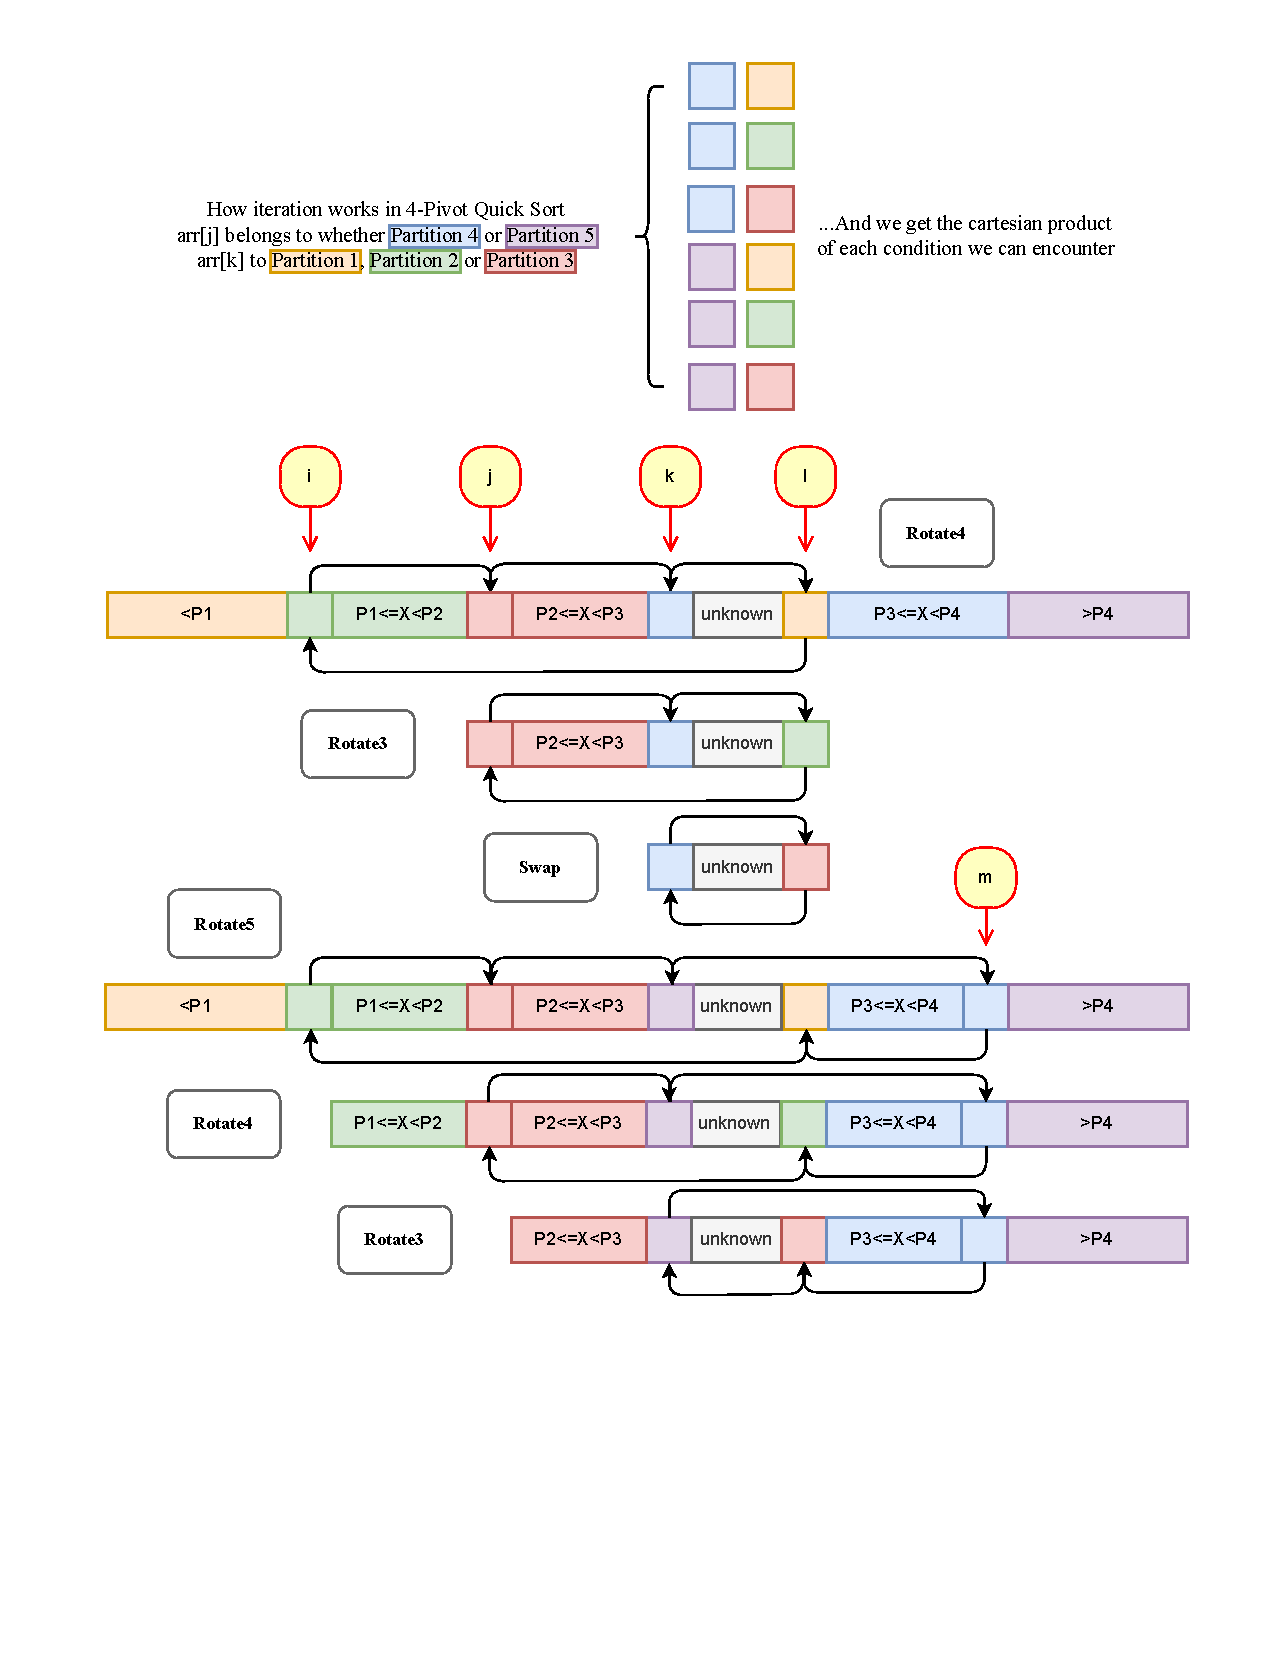
\includegraphics[width=1.5\textwidth]{4pivot.drawio.pdf}
\end{figure}




The next part of the thesis will be the implementation of the Multi-Pivot Quicksort and the BlockQuickSort,
followed by the analysis of the results and the comparisons on the performance of these algorithms.

\begin{center}
    \begin{tabular}{ |c c | c c c| }
        \hline
        Branch Misses   & Size     & Mean         & SD        & Median \\
        \hline
        1-Pivot Hoare   & 100      & 211.5502     & 0.0608    & 211.5546 \\
                        & 10k      & 3442.7053    & 2.1831    & 3442.5371 \\
                        & 10M      & 47572.1385   & 78.0503   & 47582.3149 \\
        \hline
        1-Pivot Lomuto  & 100      & 208.4046     & 0.2538    & 208.3322 \\
                        & 10k      & 3427.8026    & 2.7327    & 3427.9686 \\
                        & 10M      & 47567.6013   & 71.8560   & 47559.8385 \\
        \hline
        2-Pivot Yaro    & 100      & 218.2533     & 0.1106    & 218.2404 \\
                        & 10k      & 3626.2804    & 1.4727    & 3626.4159 \\
                        & 10M      & 50123.8209   & 72.2654   & 50129.0911 \\
        \hline
        3-Pivot Kush    & 100      & 230.1718     & 0.0892    & 230.1822 \\
                        & 10k      & 3819.6887    & 1.9794    & 3819.1637 \\
                        & 10M      & 52642.3847   & 54.1679   & 52656.3930 \\
        \hline
        4-Pivot         & 100      & 231.3465     & 0.0875    & 231.3237 \\
                        & 10k      & 3818.6932    & 2.2639    & 3818.4127 \\
                        & 10M      & 52185.5931   & 64.8748   & 52183.4357 \\
        \hline
    \end{tabular}
\end{center}

\begin{center}
    \begin{tabular}{ |c c | c c c| }
        \hline
        Cache Misses    & Size     & Mean         & SD        & Median \\
        \hline
        1-Pivot Hoare   & 100      & 0.0818       & 0.1691    & 0.0184 \\
                        & 1000     & 0.7063       & 0.8911    & 0.3544 \\
                        & 10000    & 12.4844      & 17.9061   & 7.6416 \\
        \hline
        1-Pivot Lomuto  & 100      & 0.0202       & 0.0301    & 0.0095 \\
                        & 1000     & 0.4810       & 1.0869    & 0.1625 \\
                        & 10000    & 6.5238       & 15.5592   & 2.5491 \\
        \hline
        2-Pivot Yaro    & 100      & 0.0891       & 0.1247    & 0.0557 \\
                        & 1000     & 0.6540       & 1.1752    & 0.3613 \\
                        & 10000    & 2.5734       & 1.4644    & 2.1219 \\
        \hline
        3-Pivot Kush    & 100      & 0.0244       & 0.0087    & 0.0223 \\
                        & 1000     & 0.4488       &	0.9355    & 0.1930 \\
                        & 10000    & 5.2864       & 5.4446    & 3.6768 \\
        \hline
        4-Pivot         & 100      & 0.0263       &	0.0416    &	0.0159 \\
                        & 1000     & 0.3894       &	0.6758    & 0.1691 \\
                        & 10000    & 10.9905      & 19.5457   & 5.1953 \\
        \hline
    \end{tabular}
\end{center}

\begin{center}
    \begin{tabular}{ |c c | c c c| }
        \hline
        CPU Cycles      & Size     & Mean         & SD          & Median \\
        \hline
        1-Pivot Hoare   & 100      & 8833.5322    & 3.7385      & 8832.9757 \\
                        & 1000     & 133660.4883  & 54.1056     & 133657.3592 \\
                        & 10000    & 1811140.8549 & 54157.2600  & 1793886.9439 \\
        \hline
        1-Pivot Lomuto  & 100      & 8831.1909    & 18.8702     & 8827.8629 \\
                        & 1000     & 135551.1548  & 672.3558    & 135278.5342 \\
                        & 10000    & 1823471.6121 & 1392.4438   & 1823461.0815 \\
        \hline
        2-Pivot Yaro    & 100      & 8737.9368    & 68.0570     & 8722.9634 \\
                        & 1000     & 135167.3287  &	923.0637    & 134889.7150 \\
                        & 10000    & 1814578.1631 & 2082.3356   & 1813979.9786 \\
        \hline
        3-Pivot Kush    & 100      & 8580.3270    & 3.2015      & 8579.4317 \\
                        & 1000     & 129564.1759  &	71.3810     & 129560.2397 \\
                        & 10000    & 1720134.7766 & 1718.4817   & 1719931.7412 \\
        \hline
        4-Pivot         & 100      & 8724.2381    &	1.7123      & 8724.0691 \\
                        & 1000     & 131284.4391  &	37.8241     & 131282.8758 \\
                        & 10000    & 1740851.2642 & 1393.4360   & 1740909.0583 \\
        \hline
    \end{tabular}
\end{center}
\begin{center}
    \begin{tabular}{ |c c | c c c| }
        \hline
        Time (μs)       & Size     & Mean         & SD          & Median \\
        \hline
        1-Pivot Hoare   & 100      & 2.0344       & 8.9433      & 2.0323 \\
                        & 1000     & 31.126       & 122.78      & 31.068 \\
                        & 10000    & 412.78       & 2.5557      & 411.99 \\
        \hline
        1-Pivot Lomuto  & 100      & 2.0476       & 10.402      & 2.0428 \\
                        & 1000     & 31.478       & 193.95      & 31.369 \\
                        & 10000    & 426.16       & 1.4271      & 425.74 \\
        \hline
        2-Pivot Yaro    & 100      & 8737.9368    & 68.0570     & 8722.9634 \\
                        & 1000     & 135167.3287  &	923.0637    & 134889.7150 \\
                        & 10000    & 1814578.1631 & 2082.3356   & 1813979.9786 \\
        \hline
        3-Pivot Kush    & 100      & 8580.3270    & 3.2015      & 8579.4317 \\
                        & 1000     & 129564.1759  &	71.3810     & 129560.2397 \\
                        & 10000    & 1720134.7766 & 1718.4817   & 1719931.7412 \\
        \hline
        4-Pivot         & 100      & 8724.2381    &	1.7123      & 8724.0691 \\
                        & 1000     & 131284.4391  &	37.8241     & 131282.8758 \\
                        & 10000    & 1740851.2642 & 1393.4360   & 1740909.0583 \\
        \hline
    \end{tabular}
\end{center}



\begin{thebibliography}{99}

\bibitem{HoareQuickSort} \label{HoareQuickSort} Hoare, C.A.R. (1962). Quicksort. \textit{The Computer Journal}, 5, 10-15.
\bibitem{Yaroslavskiy} \label{Yaroslavskiy} Yaroslavskiy, V. (2009). Dual-Pivot Quicksort. \textit{Proceedings of the 6th International Conference on Computer Science and Education}, 13-27.
\bibitem{Sedgewick} \label{Sedgewick} Sedgewick, R. (1978). Implementing Quicksort Programs. \textit{Communications of the ACM}, 21(10), 847-857.
\bibitem{Kushagra} \label{Kushagra} {Shrinu Kushagra, Alejandro López-Ortiz, Aurick Qiao, and J. Ian Munro. \textit{Multi-pivot quicksort: Theory and experiments.} In ALENEX, pages 47-60, 2014.}
\bibitem{Introsort} \label{Introsort} David R. Musser. \textit{Introspective Sorting and Selection Algorithms.} Software: Practice and Experience, 27(8):983-993, 1997.
\bibitem{BlockQuickSort} \label{BlockQuickSort} BlockQuicksort: How Branch Mispredictions don't affect Quicksort. \textit{Stefan Edelkamp and Armin Weiß.} 2016.
\end{thebibliography}

\end{document}